\chapter{Cooperative Pathfinding}

In this chapter, we will try to solve the problem using \textbf{Cooperative pathfinding}\cite{ARTICLE:8}.
There are some drawbacks related to this approach that we will see at the end of chapter and 
ways to resolve it.
When a single unit pathfinds through a map, basic A* search is perfectly adequate. But
when multiple units are moving at the same time, this approach can break down, often
with frustrating consequences for the player.

\section{The problem with A*}
A* search is used to find
the shortest path to the destination for each unit (agent in case of flatland environment). This search ignores the
presence of other units, or perhaps treats them as stationary obstacles. If a collision is
imminent, the units involved will re-search and select a new path.

\vspace {\baselineskip}
In case of \textbf{cooperative pathfinding}, A* search is still used, but in a way that takes account of other
agents’ movements. The only requirement is that agents can communicate their planned paths which is always
possible in case of flatland environment. This is generally
most appropriate for agents on the same side; agents 
units will not usually be so cooperative. 
Non-cooperative pathfinding raises the tricky issue of path prediction, and
isn’t discussed here as it is not applicable to our flatland problem.

\section{The Fourth Dimension}
To tackle the cooperative pathfinding problem, the search algorithm needs to have full
knowledge of both obstacles and agents. However, when agents move around there is no
satisfactory way to represent their routes on a stationary map. To overcome this problem,
we extend the map to include a fourth dimension: time. We will call the original map the
space map and the new, extended map the space-time map.
The \textbf{space map} consists of a three-dimensional grid of
locations and orientation (x, y,orientation). The \textbf{space-time} map consists of a four-dimensional grid
of cells: Cell(x, y, orientation, t).

\vspace{\baselineskip}

In flatland environment, agent have 5 actions: do nothing, deviate left (if possible), go forward, deviate right (if possible), stop.
Executing forward (when the agent is facing North) corresponds to moving a agent through the space-time map from
Cell(x, y, North , t) to Cell(x, y + 1, North , t + 1).All five actions have a cost
of one, corresponding to their duration. Once the agent reaches the target, agent will 
disappear. A* search can now be used on the space-time map. The goal of the agent is to reach the
destination at any time. A* will find the route that achieves this goal with the lowest cost.

\section{Reservation Table}
Once a agent has chosen a path, it needs to make sure that other agents know to avoid the
cells along its path. This is achieved by marking each agent into a \textbf{reservation table}. This is
a straightforward data structure containing an entry for every cell of the space-time map \textbf{excluding the orientation}.
Each entry specifies whether the corresponding cell is available or reserved. Once an
entry is reserved, it is illegal for any other agent to move into that cell. The reservation acts
like a transient obstacle, blocking off a location for a single time-step in the future.

\vspace{\baselineskip}
Using a reservation table and a space-time map, we are able to solve the cooperative
pathfinding problem. Each agent pathfinds to its destination using space-time A*, and then
marks the path into the reservation table. Subsequent agents will avoid any
reserved cells, giving exactly the coordinated behavior that we desire.
Note, a cell is reserved when some location is occupied at some time. Orientation does not have 
any role here.

\begin{figure}[h]
    \centering
    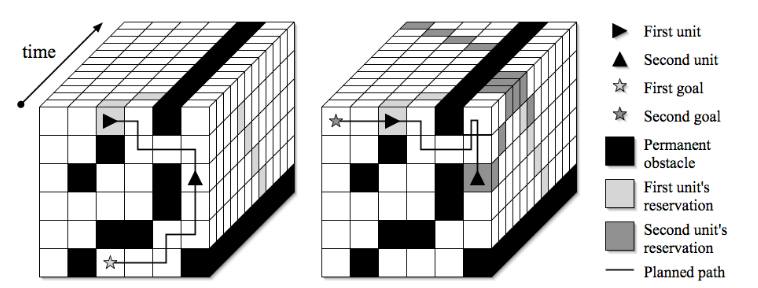
\includegraphics[width=1.0\textwidth]{Cooperative1}
    \caption{ Two agents pathfinding cooperatively. (A) The first agent searches for a path and
    marks it into the reservation table. (B) The second agent searches for a path, taking account
    of existing reservations, and also marks it into the reservation table. Orientation is not shown in 
    this example.\cite{ARTICLE:8}}
    \label{image-myimage2}
\end{figure}

We are reserving one cell in the reservation table for the agent. But it can lead to deadlock when executing.
Unfortunately, this way of using the reservation table doesn’t prevent two agents crossing
through each other, head to head. If one agent has reserved (x, y, t) and (x + 1, y, t + 1),
there is nothing to stop a second agent from reserving (x + 1, y, t) and (x, y, t + 1). Note orientation 
is not used in case of reservation table. This
problem can be avoided by making \textbf{two reservations} for each location involved in the
action, one at time t and one at time t + 1. Alternatively, head to head collisions can be
explicitly identified and marked as illegal actions. We will be making two reservations for each location 
in our work as it is able to avoid the deadlock completely. We now have a complete algorithm for cooperative pathfinding.

\section{Choosing heuristic}
The performance of A* depends upon the choice of heuristic. With the search space
extended by an extra dimension, the choice of heuristic becomes even more important.

\subsection{Manhattan distance heuristic}
For grid-based maps, the Manhattan distance is often used as a heuristic. It is simply the
sum of the x and y distances to the destination. It provides a good estimate of the time to
reach the destination on an open map. However, if the shortest path to the destination is
circuitous, then the Manhattan distance becomes a poor estimate.

\vspace{\baselineskip}
During A* search, new locations are kept on the open list and explored locations are kept
on the closed list. At each step, the most promising location is selected from the open list
according to its f value. The f value estimates the total distance to the destination, passing
through that location. It is the sum of g, the distance traveled by A* to reach the location,
and h, the heuristic distance from the location to the destination.

Using the Manhattan distance heuristic, many locations on the map can have an f value
that is less than the true distance to the destination. For example, the map in given figure (not showing orientation dimension 
to make things simple)
shows the f values for all locations visited by spatial A*. Almost the entire map has been
explored before the destination is found, a phenomenon known as \textbf{flooding}.

\begin{figure}[h]
    \centering
    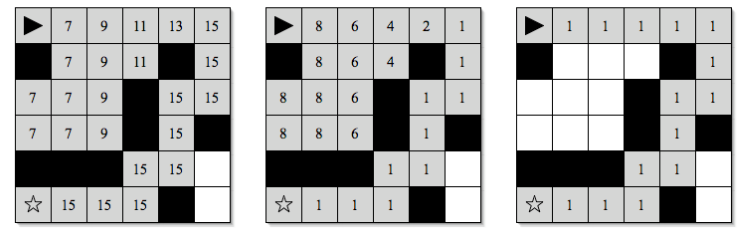
\includegraphics[width=1.0\textwidth]{cooperative2}
    \caption{The Manhattan distance heuristic can be inefficient. (A) Flooding occurs in
    spatial A* when the f values (shown) at many locations are lower than at the destination.
    (B) The number of visits to each location (shown) can be high during space-time A*. (C)
    Using the true distance heuristic, the number of visits to each location (shown) is optimal.\cite{ARTICLE:8}}
    \label{image-myimage2}
\end{figure}

Now consider what happens if we use the Manhattan distance in a space-time map.
Again, it will work well on an open map. But take a look at the equivalent map in Figure, which shows
 the number of times each location is explored by space-time A*. Not
only will space-time A* explore many more locations at the time of each deviation, it will
explore those locations at later times too. This is because pausing, or returning to a
previous location, appears more promising than moving away from the destination. In
other words, \textbf{the problem has been magnified many times}.

\subsection{True distance heuristic}
We will use true distance heuristic as our heuristic for space-time search. True distance heusristic is 
the shortest distance to the destination, taking account of obstacles, but ignoring agents.
True distance from each location and orientation to each target is pre calculated and stored to make the 
algorithm faster. When using true distance heuristic in case of cooperative pathfinding, the algorithm is 
known as \textbf{Hierarchical Cooperative A*}

\subsubsection{Consistency}
An admissible heuristic never overestimates the distance to the goal. A* search with an
admissible heuristic is guaranteed to find the shortest path. However, there is a stronger
property, known as consistency. A \textbf{consistent heuristic maintains the property
h(A) $\leq$ cost(A, B) + h(B) between all locations A and B}. In other words, the estimated
distance doesn’t jump around between the locations along a path. Both manhattan and true distance heuristic
are consistent.


\section{Results}
We implemented the cooperative A* (both manhattan and true distance heuristic) on flatland environment 
having both only one cell reserved (at time t) and two cell reserved (at time t and t+1).

\subsection{Cooperative A* with only cell reserved at t}
When only one cell is reserved at time t, the results are very bad as \textbf{most of the agents ended in 
deadlock}. In case of problem instance 1, only 2 out of 10 agents completed their journey. Rest ended in deadlock.
In case of problem instance 2, 13 out of 20 agents completed their journey. This is still high because problem 
instance 2, have multiple paths from each location and orientation to there target.
In case of problem instance 3 (real life example), only 6 out of 100 agents are able to complete journey.
Clearly, this algorithm is not good. 

\subsection{Cooperative A* with cell reserved at t and t+1}
The results in this case are very good, as all the agents are able to complete their journey with great cooperation.
I am attaching a video showing the great cooperation between agents. One thing to notice is \textbf{path length}
for each agent after they complete their journey. In case of problem instance 1, agents 6 and 8 take much larger path
compared to shortest path. In case of problem instance 2, since there are so many paths from given location 
and orientation to the target, actual path taken by the agent and shortest path are almost of same length.
In case of problem instance 3 (real life example), as the agent number increases they take longer and longer routes.
This is because the agent with less order number have already made reservations and agent with higher order number 
have to take alternate path other than the best path. In fact the extent of deviation from the 
shortest path shows the cooperation between the agents. So, with agent with less order number have 
\textbf{higher priority}. So we can assign priority to the trains based on there order number.
Although this is not very good.
\begin{figure}[h]
    \centering
    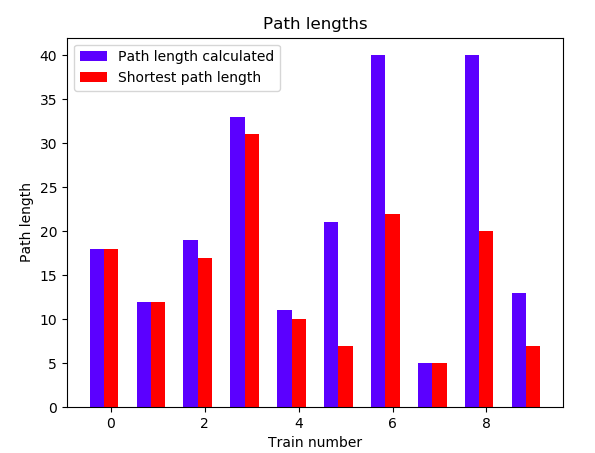
\includegraphics[width=0.5\textwidth]{cooperative3}
    \caption{Pathlength (problem instance 1)}
    \label{image-myimage2}
\end{figure}

\begin{figure}[h]
    \centering
    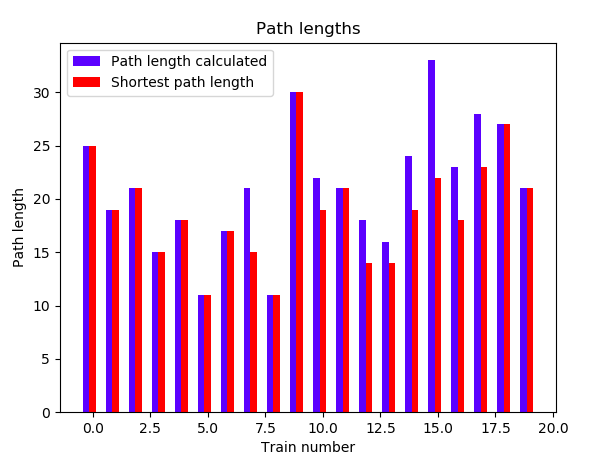
\includegraphics[width=0.5\textwidth]{cooperative4}
    \caption{Pathlength (problem instance 2)}
    \label{image-myimage2}
\end{figure}

\begin{figure}[H]
    \centering
    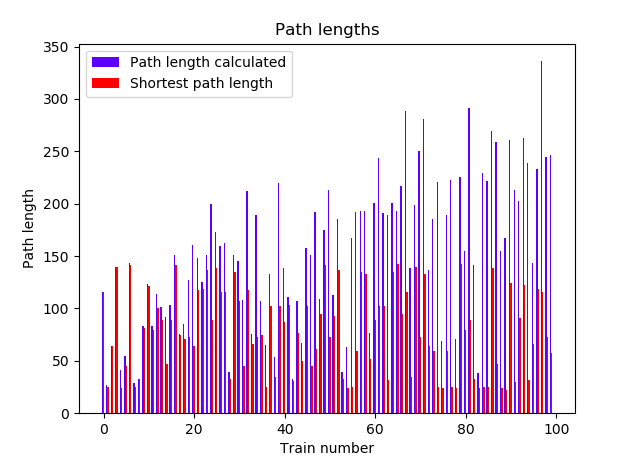
\includegraphics[width=0.8\textwidth]{cooperative5}
    \caption{Pathlength (problem instance 1)}
    \label{image-myimage2}
\end{figure}

\section{Drawbacks}
Hierarchical cooperative A* works really good on flatland environment, but this algorithm is deterministic.
This mean, if we include stochasticity into the system, by making agent malfunction, this algorithm is likely 
to break. To solve this issue, instead of finding the path upto the target, agent can find path upto certain 
depth and then once completed that depth, can resume search. This will be more robust to stochasticity in 
environment. This algorithm is called \textbf{Windowed Hierarchical cooperative A* (WHCA)}.
Also, in Hierarchical cooperative A*, priority is already introduced depending on the agent order. This can be resolved searching 
the path upto fixed depth, follow the path and then change order. This way each agent will have higher priority at some point 
of time and hence resolving the issue. We can also try to combine this algorithm with some RL algorithm to make it 
more robust to the environment with high stochasticity.